\chapter{Espectrometria de massas e espectroscopia atômica}\label{ch:b2:mass-spec-atomic}

Os fogos de artifício são vermelhos com sais de estrôncio, verdes com sais de bário, amarelos com o
sódio: uma chama transforma os átomos em luz de cores que os identificam. Um espectrômetro de massas,
de aparência mais modesta, pesa moléculas isoladas, as classifica por seus isótopos e as quebra em
pedaços cujas massas dizem como elas foram construídas. As duas técnicas respondem à pergunta ``o que
há nesta amostra, e quanto?'' a partir de quantidades muito pequenas, a primeira para as moléculas, a
segunda para os elementos.

\begin{omfigure}
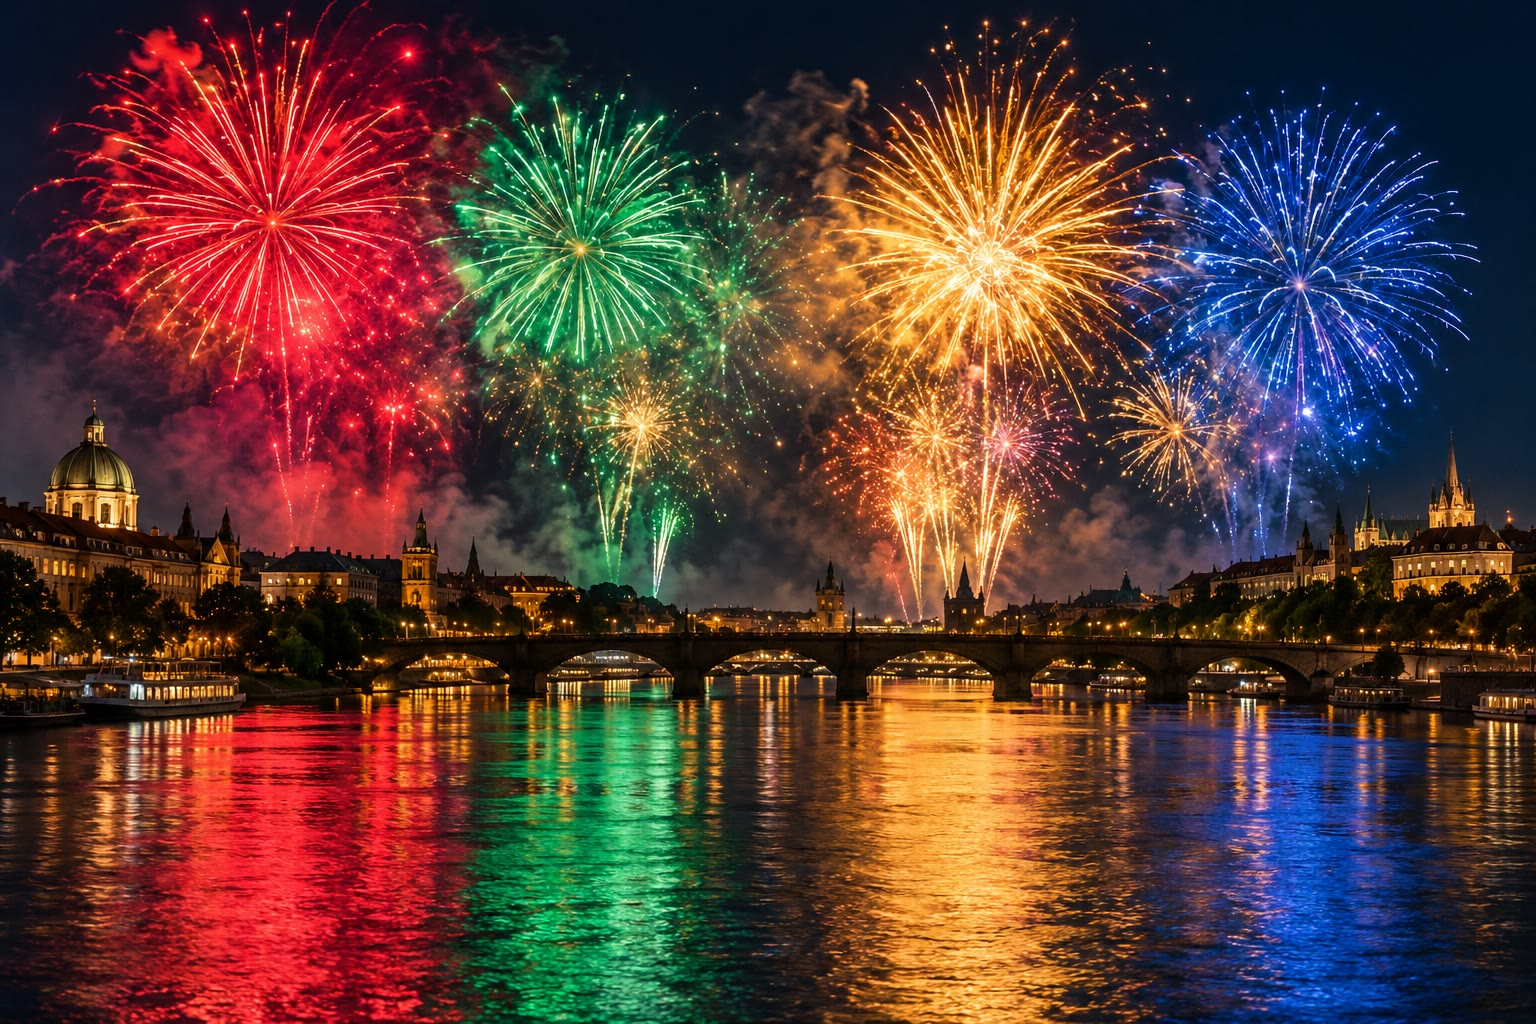
\includegraphics[width=0.58\linewidth]{images/book3/ai/b2-32-fireworks.jpg}

{\small Fogos de artifício sobre um rio (ilustração). O amarelo do sódio é a luz de seus átomos; os
vermelhos e verdes intensos vêm em grande parte de pequenas moléculas de estrôncio e de bário formadas
na chama.}
\end{omfigure}

\begin{recall}
O volume escolar: os isótopos e suas abundâncias. O volume do 1.º ano: níveis de energia e raias
espectrais, absorbância e lei de Beer--Lambert, carbocátions e radicais, o grau de insaturação.
\Cref{ch:b2:chromatography}: a \omterm{def:b2:chromatography:techniques}{cromatografia gasosa}, que muitas vezes alimenta um espectrômetro de massas.
\end{recall}

\section{O espectrômetro de massas}

\begin{definition}[Espectrometria de massas]\label{def:b2:mass-spec-atomic:spectrum}
A \emph{espectrometria de massas}\index{espectrometria de massas} transforma as moléculas de uma amostra em íons gasosos,
separa os íons segundo sua \emph{razão massa/carga}\index{razao massa/carga@razão massa/carga} $m/z$
(a massa em unidades de massa atômica unificada dividida pelo número de cargas) e os conta. O
\emph{espectro de massas}\index{espectro de massas} representa a abundância dos íons em função de $m/z$, em geral como
intensidades relativas; seu pico mais intenso, fixado em 100, é o \emph{pico base}\index{pico base}.
\end{definition}

Um espectrômetro tem três partes. A fonte produz os íons. Na ionização por elétrons (EI), o vapor da
amostra atravessa um feixe de elétrons de \qty{70}{eV}, que arrancam um elétron das moléculas e as
deixam com um excesso de energia, de modo que muitas se quebram. Na ionização por eletrospray (ESI), uma
solução é pulverizada a partir de uma agulha carregada; à medida que as gotículas evaporam, moléculas as
deixam levando um próton a mais (ou um íon sódio), intactas: o método preferido para moléculas grandes e
frágeis. O analisador então classifica os íons, e um detector os conta.

\begin{omfigure}
\begin{tikzpicture}[x=1cm, y=1cm]
\draw[black!70, fill=omDef!10, rounded corners=2pt] (0,-0.6) rectangle (1.6,0.6);
\node[font=\small, align=center] at (0.8,0) {fonte\\de íons};
\draw[black!70] (2.0,-0.7) -- (2.0,0.7); \draw[black!70] (2.4,-0.7) -- (2.4,0.7);
\node[font=\footnotesize] at (2.2,1.0) {grades, $U$};
\draw[black!70] (2.6,-0.5) rectangle (8.4,0.5);
\node[font=\small] at (5.6,0.8) {tubo sem campo, comprimento $L$};
\draw[black!70, fill=black!15] (8.5,-0.6) rectangle (8.8,0.6);
\node[font=\small, align=center] at (9.6,0) {detector};
\foreach \x/\c in {3.4/omThm, 4.6/omDef, 6.3/omMeth}{\fill[\c] (\x,0) circle (0.1);}
\draw[->, thick] (6.6,0) -- (7.4,0);
\node[font=\footnotesize, align=center] at (5.5,-0.85) {os íons leves voam à frente, os pesados se atrasam};
\end{tikzpicture}
\par\vspace{4pt}

{\small Um analisador de tempo de voo (esquema). Os íons acelerados pela mesma diferença de potencial
$U$ saem com a mesma energia cinética; no tubo de voo os mais leves viajam mais depressa e chegam
primeiro ao detector.}
\end{omfigure}

\begin{proposition}[Tempo de voo]\label{prop:b2:mass-spec-atomic:time-of-flight}
Um íon de massa $m$ e carga $ze$, acelerado a partir do repouso por uma diferença de potencial $U$,
atravessa um tubo sem campo de comprimento $L$ em
\begin{equation*}
t = L\sqrt{\frac{m}{2zeU}}:
\end{equation*}
o tempo de voo cresce como a raiz quadrada de $m/z$.
\end{proposition}

\begin{proof}
A conservação da energia no campo acelerador dá $\tfrac12mv^2 = zeU$, logo $v = \sqrt{2zeU/m}$, e
o tubo é atravessado a velocidade constante: $t = L/v$.
\end{proof}

Outros analisadores classificam os íons de outro modo: um quadrupolo deixa passar apenas os íons de um
$m/z$ de cada vez, selecionados por tensões oscilantes em quatro barras; um setor magnético curva os íons
em círculos cujo raio depende de seu momento linear. Em todos eles só $m/z$ é medido; a maioria dos íons
produzidos por EI leva uma carga, de modo que $m/z$ é simplesmente sua massa.

\section{O íon molecular}

\begin{definition}[Íons molecular e fragmentos]\label{def:b2:mass-spec-atomic:molecular-ion}
O \emph{íon molecular}\index{ion molecular@íon molecular} $\mathrm M^{+\bullet}$ é o cátion radical formado quando uma
molécula perde um elétron; seu $m/z$ é a massa molar da molécula formada pelos isótopos mais
abundantes. Um \emph{íon fragmento}\index{ion fragmento@íon fragmento} provém do íon molecular pela ruptura de
ligações.
\end{definition}

O \omterm{def:b2:mass-spec-atomic:molecular-ion}{íon molecular} dá a massa molecular, o primeiro dado sobre uma substância desconhecida. Às vezes ele é
fraco ou ausente em EI, quando o \omterm{def:b2:mass-spec-atomic:molecular-ion}{íon molecular} se quebra fácil demais; o eletrospray, que dá $[\mathrm M +
\mathrm H]^+$ uma unidade acima, então o confirma.

\begin{definition}[Regra do nitrogênio]\label{def:b2:mass-spec-atomic:nitrogen-rule}
A \emph{regra do nitrogênio}\index{regra do nitrogenio@regra do nitrogênio} afirma que uma molécula tem massa nominal ímpar (a soma
dos números de massa de seus isótopos mais abundantes) se e somente se contém um número ímpar de átomos
de nitrogênio.
\end{definition}

\begin{proposition}[Validade da regra do nitrogênio]\label{prop:b2:mass-spec-atomic:nitrogen-rule}
A \omterm{def:b2:mass-spec-atomic:nitrogen-rule}{regra do nitrogênio} vale para toda molécula sem elétrons desemparelhados construída a partir de C, H,
N, O, S e dos halogênios.
\end{proposition}

\begin{proof}
As massas nominais são pares para C (12), N (14), O (16) e S (32), ímpares para H (1) e os halogênios (19,
35, 79, 127). As valências são pares para C, O e S, ímpares para H, N e os halogênios. Em uma molécula
sem elétrons desemparelhados, cada ligação usa uma valência de cada um de seus dois átomos, de modo que a
soma de todas as valências é par, e o número de átomos de valência ímpar, $n_{\ce{H}} + n_{\ce{X}} + n_{\ce{N}}$, é
par. A paridade da massa nominal é a de $n_{\ce{H}} + n_{\ce{X}}$, que é portanto a de
$n_{\ce{N}}$.
\end{proof}

\begin{definition}[Perfil isotópico]\label{def:b2:mass-spec-atomic:isotope-pattern}
O \emph{perfil isotópico}\index{perfil isotopico@perfil isotópico} de um íon é o grupo de picos em $M$, $M+1$,
$M+2$, \dots\ produzidos pelas moléculas que contêm isótopos mais pesados, com intensidades
proporcionais às abundâncias dessas formas isotópicas.
\end{definition}

\begin{proposition}[O pico $M+1$]\label{prop:b2:mass-spec-atomic:m-plus-one}
Para um íon com $n_C$ átomos de carbono e nenhum outro elemento com um isótopo $+1$ significativo,
\begin{equation*}
\frac{I(M+1)}{I(M)} \approx n_C\,\frac{a_{13}}{a_{12}} \approx n_C \times 1.1~\%,
\end{equation*}
onde $a_{12} = 0.989$ e $a_{13} = 0.011$ são as frações em quantidade dos dois isótopos do carbono.
% ledger: iso:C12, iso:C13
\end{proposition}

\begin{proof}
A probabilidade de que todos os $n_C$ carbonos sejam \ce{^{12}C} é $a_{12}^{n_C}$; a de que exatamente um
seja \ce{^{13}C} é $n_C\,a_{13}a_{12}^{n_C - 1}$ (lei binomial). A razão é $n_C\,a_{13}/a_{12}$, e as
outras contribuições (dois \ce{^{13}C}, \ce{^2H}, \ce{^{15}N}) são menores por um fator da ordem de
$a_{13}$ ou menos.
\end{proof}

\begin{proposition}[Cloro e bromo]\label{prop:b2:mass-spec-atomic:halogen-patterns}
Para um íon com $p$ átomos de cloro e $q$ de bromo, as intensidades de $M$, $M+2$, $M+4$, \dots\ são
os coeficientes do desenvolvimento de $(a_{35} + a_{37}x)^p(a_{79} + a_{81}x)^q$ em potências de $x$,
cada potência de $x$ representando 2 unidades de massa. Com $a_{35} = 0.758$, $a_{37} = 0.242$, $a_{79} = 0.5069$ e
$a_{81} = 0.4931$, um cloro dá $M : M+2 \approx 3 : 1$ e um bromo $\approx 1 : 1$.
% ledger: iso:Cl35, iso:Cl37, iso:Br79, iso:Br81
\end{proposition}

\begin{proof}
Cada átomo de halogênio é, de modo independente, o isótopo leve ou o pesado, que acrescenta 2 à massa. A
probabilidade de um dado número $j$ de átomos pesados é o coeficiente de $x^j$ no produto de um fator por
átomo, que é o desenvolvimento enunciado (a lei binomial, por elemento).
\end{proof}

\begin{omfigure}
\pgfplotsset{clu/.style={width=0.25\linewidth, height=3.3cm, ybar, bar width=5pt, ymin=0, ymax=118,
  xmin=-1.2, xmax=5.2, xtick={0,2,4}, xticklabels={$M$,$M\!+\!2$,$M\!+\!4$},
  tick label style={font=\tiny}, ytick=\empty, axis x line=bottom, axis y line=none,
  title style={font=\small, yshift=-4pt}, nodes near coords, nodes near coords style={font=\tiny},
  point meta=y, every node near coord/.append style={/pgf/number format/fixed, /pgf/number format/precision=0}}}
\begin{tikzpicture}
\begin{axis}[clu, title={Cl}]
\addplot[fill=omDef!55, draw=omDef, y filter/.expression={y==0 ? nan : y}] table[x=off, y=Cl] {figdata/out/bachelor-2-mass-spectra-a.dat};
\end{axis}
\end{tikzpicture}\hfill
\begin{tikzpicture}
\begin{axis}[clu, title={Cl$_2$}]
\addplot[fill=omDef!55, draw=omDef] table[x=off, y=Cl2] {figdata/out/bachelor-2-mass-spectra-a.dat};
\end{axis}
\end{tikzpicture}\hfill
\begin{tikzpicture}
\begin{axis}[clu, title={Br}]
\addplot[fill=omThm!45, draw=omThm, y filter/.expression={y==0 ? nan : y}] table[x=off, y=Br] {figdata/out/bachelor-2-mass-spectra-a.dat};
\end{axis}
\end{tikzpicture}\hfill
\begin{tikzpicture}
\begin{axis}[clu, title={Br$_2$}]
\addplot[fill=omThm!45, draw=omThm] table[x=off, y=Br2] {figdata/out/bachelor-2-mass-spectra-a.dat};
\end{axis}
\end{tikzpicture}\hfill
\begin{tikzpicture}
\begin{axis}[clu, title={ClBr}]
\addplot[fill=omMeth!45, draw=omMeth] table[x=off, y=ClBr] {figdata/out/bachelor-2-mass-spectra-a.dat};
\end{axis}
\end{tikzpicture}

{\small \omterm{def:b2:mass-spec-atomic:isotope-pattern}{Perfis isotópicos} de íons que contêm cloro e bromo, calculados a partir das abundâncias
isotópicas (\cref{prop:b2:mass-spec-atomic:halogen-patterns}); o pico mais intenso de cada grupo é
fixado em 100. Os perfis são impressões digitais: 3 : 1 para um cloro, 1 : 1 para um bromo, 1 : 2 : 1
para dois bromos.}
% figdata: bachelor-2/mass-spectra.py part a
\end{omfigure}

\begin{definition}[Massa exata]\label{def:b2:mass-spec-atomic:exact-mass}
A \emph{massa monoisotópica}\index{massa monoisotopica@massa monoisotópica} de um íon é a soma das massas exatas de seus
isótopos mais abundantes (\ce{^{12}C} = 12 exatamente, \ce{^1H} = 1.007825, \ce{^{16}O} = 15.994915,
\ce{^{14}N} = 14.003074 u). A \emph{espectrometria de massas de alta resolução}\index{espectrometria de massas de alta resolucao@espectrometria de massas de alta resolução}
mede $m/z$ com alguns milésimos de unidade ou melhor, o suficiente para distinguir íons de mesma
massa nominal mas de fórmulas diferentes.
% ledger: mass:C12, mass:H1, mass:O16, mass:N14
\end{definition}

\begin{proposition}[Poder de resolução]\label{prop:b2:mass-spec-atomic:resolving}
Dois íons de massas $m$ e $m + \Delta m$ são separados por um analisador de poder de resolução pelo menos
$R = m/\Delta m$. Na massa nominal 28, separar \ce{CO+} (27.9949) de \ce{N2+} (28.0061) exige $R
\approx 2.5 \times 10^3$; separar \ce{N2+} de \ce{C2H4+} (28.0313), $R \approx 1.1 \times 10^3$.
\end{proposition}

\begin{proof}
O poder de resolução é definido como $m/\Delta m$ para o menor $\Delta m$ que o analisador separa. As
massas exatas decorrem das massas isotópicas: $12 + 15.994915$, $2 \times 14.003074$, $24 + 4 \times
1.007825$; então $28/(28.0061 - 27.9949) \approx 2.5 \times 10^3$ e $28/(28.0313 - 28.0061) \approx
1.1 \times 10^3$.
\end{proof}

\section{A fragmentação}

O \omterm{def:b2:mass-spec-atomic:molecular-ion}{íon molecular} produzido por EI leva muito mais energia do que qualquer ligação precisa para se romper, e
ele se quebra pelos caminhos que dão os produtos mais estáveis: cátions estabilizados, pequenas moléculas
neutras estáveis ou radicais. Os fragmentos são lidos como perdas a partir de $M$ (15 para \ce{CH3}, 29
para \ce{C2H5} ou \ce{CHO}, 18 para a água, 28 para CO ou o eteno) e como íons característicos.

\begin{definition}[Duas fragmentações]\label{def:b2:mass-spec-atomic:fragmentation}
Em uma \emph{clivagem $\alpha$}\index{clivagem alfa@clivagem $\alpha$}, uma ligação com o carbono vizinho de um
heteroátomo ou de uma carbonila se rompe, deixando um cátion estabilizado pelo par não ligante do
heteroátomo (um \omterm{def:b2:aromatic-substitution:friedel-crafts}{íon acílio} $\mathrm{R{-}C{\equiv}O^+}$ para uma cetona, um íon imínio para uma amina). O
\emph{rearranjo de McLafferty}\index{rearranjo de McLafferty} de um composto carbonílico transfere um hidrogênio do
carbono $\gamma$ para o oxigênio carbonílico e rompe a ligação $\alpha$--$\beta$, liberando um alceno e
um cátion radical de \omterm{def:b2:enolates-aldol:tautomerism}{enol}.
\end{definition}

\begin{omfigure}
\begin{tikzpicture}
\begin{axis}[width=0.48\linewidth, height=4.6cm, xmin=10, xmax=80, ymin=0, ymax=118,
  xlabel={$m/z$}, ylabel={intensidade relativa}, label style={font=\small}, tick label style={font=\scriptsize},
  title={\small butan-2-ona}, ycomb, xtick={15,29,43,57,72}]
\addplot[omDef, thick] table[x=mz, y=I] {figdata/out/bachelor-2-mass-spectra-b.dat};
\node[font=\tiny, anchor=south] at (axis cs:43,100) {43};
\node[font=\tiny, anchor=south] at (axis cs:72,25) {72};
\node[font=\tiny, anchor=south] at (axis cs:57,8) {57};
\node[font=\tiny, anchor=south] at (axis cs:29,17) {29};
\end{axis}
\end{tikzpicture}\hfill
\begin{tikzpicture}
\begin{axis}[width=0.48\linewidth, height=4.6cm, xmin=10, xmax=140, ymin=0, ymax=118,
  xlabel={$m/z$}, ylabel={intensidade relativa}, label style={font=\small}, tick label style={font=\scriptsize},
  title={\small 1-bromopropano}, ycomb, xtick={27,43,79,107,122}]
\addplot[omThm, thick] table[x=mz, y=I] {figdata/out/bachelor-2-mass-spectra-c.dat};
\node[font=\tiny, anchor=south] at (axis cs:43,100) {43};
\node[font=\tiny, anchor=south] at (axis cs:123,9) {122, 124};
\node[font=\tiny, anchor=south] at (axis cs:27,26) {27};
\node[font=\tiny, anchor=south east] at (axis cs:40.5,31) {41};
\end{axis}
\end{tikzpicture}

{\small Espectros de ionização por elétrons (dados do NIST WebBook). Butan-2-ona: \omterm{def:b2:mass-spec-atomic:molecular-ion}{íon molecular} em 72;
as clivagens $\alpha$ dão os \omterm{def:b2:aromatic-substitution:friedel-crafts}{íons acílio} \ce{CH3CO+} (43, \omterm{def:b2:mass-spec-atomic:spectrum}{pico base}) e \ce{C2H5CO+} (57). 1-bromopropano:
o \omterm{def:b2:mass-spec-atomic:molecular-ion}{íon molecular} é um par 1 : 1 em 122 e 124 (\ce{^{79}Br}, \ce{^{81}Br}); a perda do átomo de bromo
deixa \ce{C3H7+} em 43, o \omterm{def:b2:mass-spec-atomic:spectrum}{pico base}.}
% figdata: bachelor-2/mass-spectra.py parts b, c
% ledger: ms:butanone, ms:bromopropane
\end{omfigure}

\begin{omfigure}
\setchemfig{atom sep=1.8em}
\schemestart
\chemfig{[:-30]\chemabove{O}{\scriptstyle +\bullet}?[a]=[:-90]C(-[:-150]H_3C)-[:-30]CH_2-[:30]CH_2-[:90]CH_2-[:150]H?[a,1,{dash pattern=on 1pt off 1.5pt}]}
\arrow{->}[,1.0]
\chemfig{CH_2=C(-[2]OH)-CH_3}\,$^{+\bullet}$
\+
\chemfig{CH_2=CH_2}
\schemestop
\par\vspace{6pt}

{\small O \omterm{def:b2:mass-spec-atomic:fragmentation}{rearranjo de McLafferty} da pentan-2-ona, desenhado por meio de seu arranjo cíclico de seis
membros: o hidrogênio do carbono $\gamma$ passa para o oxigênio, a ligação $\alpha$--$\beta$ se rompe,
o eteno sai, e o cátion radical do \omterm{def:b2:enolates-aldol:tautomerism}{enol} da propanona fica em $m/z$ 58.}
\end{omfigure}

\begin{proposition}[Exigência de McLafferty]\label{prop:b2:mass-spec-atomic:mclafferty}
Um \omterm{def:b2:mass-spec-atomic:fragmentation}{rearranjo de McLafferty} exige um hidrogênio no carbono $\gamma$. Ele libera um alceno e deixa um
cátion radical cuja massa tem a paridade da massa molecular (par para um composto sem
nitrogênio).
\end{proposition}

\begin{proof}[Raciocínio]
O hidrogênio é transferido por meio de um arranjo cíclico de seis membros formado pelo oxigênio, o
carbono carbonílico, os carbonos $\alpha$, $\beta$ e $\gamma$ e o próprio hidrogênio: só um hidrogênio
$\gamma$ alcança o oxigênio sem tensão. O íon formado conserva o grupo carbonila, o carbono $\alpha$ e o
hidrogênio transferido; o que sai é um alceno, uma molécula neutra de massa par, de modo que o íon
conserva a paridade de $M$, o que o distingue dos cátions de massa ímpar produzidos pelas clivagens simples.
\end{proof}

\begin{method}[Ler um espectro de massas]\label{met:b2:mass-spec-atomic:read-ms}
\begin{enumerate}
  \item Encontre o \omterm{def:b2:mass-spec-atomic:molecular-ion}{íon molecular} (maior $m/z$ do agrupamento principal, com perdas plausíveis abaixo dele).
  \item Leia seu \omterm{def:b2:mass-spec-atomic:isotope-pattern}{perfil isotópico}: Cl, Br, S; o pico $M+1$ dá o número de carbonos.
  \item Aplique a \omterm{def:b2:mass-spec-atomic:nitrogen-rule}{regra do nitrogênio}; proponha fórmulas e seu grau de insaturação.
  \item Leia as perdas a partir de $M$ e os íons característicos (43 \ce{CH3CO+} ou \ce{C3H7+}, 77
        \ce{C6H5+}, 91 \ce{C7H7+}, 105 \ce{C6H5CO+}); procure íons de McLafferty de massa par.
  \item Proponha estruturas; verifique que cada pico importante é explicado.
\end{enumerate}
\end{method}

\section{A espectroscopia atômica}

Os átomos não têm vibrações nem rotações; seus espectros são raias finas, uma por transição entre níveis
eletrônicos, em comprimentos de onda característicos do elemento. O amarelo de uma chama de sódio é o
par de raias em \qty{589.0}{nm} e \qty{589.6}{nm}; o carmim do lítio, uma raia em \qty{670.8}{nm};
a raia mais forte dos átomos de estrôncio fica em \qty{460.7}{nm} e a dos íons de bário em
\qty{455.4}{nm}, no azul: os vermelhos e verdes dos fogos de artifício vêm sobretudo de moléculas desses
metais, não de seus átomos.
% ledger: asd:NaD2, asd:NaD1, asd:Li671, asd:Sr461, asd:Ba455

\begin{definition}[Espectrometrias atômicas]\label{def:b2:mass-spec-atomic:atomic}
Na \emph{espectrometria de emissão atômica}\index{espectrometria de emissao atomica@espectrometria de emissão atômica} a amostra é atomizada e
excitada em uma chama ou um plasma, e mede-se a intensidade de uma raia de emissão do elemento. Na
\emph{espectrometria de absorção atômica}\index{espectrometria de absorcao atomica@espectrometria de absorção atômica} (EAA) a amostra é
atomizada em uma chama ou um forno de grafite e mede-se a absorbância dos átomos em uma raia de
ressonância, emitida por uma \emph{lâmpada de cátodo oco}\index{lampada de catodo oco@lâmpada de cátodo oco} cujo cátodo é feito do
próprio elemento. Em um \emph{plasma indutivamente acoplado}\index{plasma indutivamente acoplado} (ICP), o argônio
aquecido por um campo de radiofrequência a vários milhares de kelvins atomiza e ioniza a amostra; o
plasma alimenta um espectrômetro de emissão (ICP-OES) ou um espectrômetro de massas (ICP-MS).
\end{definition}

\begin{omfigure}
\begin{tikzpicture}[x=1cm, y=1cm, box/.style={draw=black!70, rounded corners=2pt, fill=white,
  font=\small, align=center, minimum height=0.8cm, inner sep=3pt}]
\node[box] (lamp) at (0,0) {lâmpada de\\cátodo oco (Cu)};
\shade[top color=omThm!60, bottom color=omThm!10] (2.6,-0.25) -- (3.3,-0.25) -- (3.15,0.75) -- (2.75,0.75) -- cycle;
\draw[black!70, fill=black!15] (2.4,-0.45) rectangle (3.5,-0.25);
\node[font=\footnotesize] at (2.95,-0.75) {chama (átomos)};
\node[box] (mono) at (6.1,0) {mono-\\cromador};
\node[box] (det) at (8.5,0) {detector};
\node[box] (data) at (10.8,0) {absorbância};
\draw[->, thick, omDef] (lamp.east) -- (mono.west);
\draw[->, thick] (mono) -- (det); \draw[->, thick] (det) -- (data);
\node[font=\footnotesize, omDef] at (4.4,0.3) {$I_0 \to I$};
\end{tikzpicture}
\par\vspace{4pt}

{\small Um espectrômetro de absorção atômica (esquema). A lâmpada emite as raias do próprio cobre, entre
elas a raia de ressonância em \qty{324.75}{nm}; os átomos de cobre na chama a absorvem, e o
monocromador isola essa raia para o detector.}
% ledger: asd:Cu325
\end{omfigure}

\begin{proposition}[A absorção atômica é quantitativa]\label{prop:b2:mass-spec-atomic:aas}
Em uma faixa de concentrações, a absorbância medida em uma raia de ressonância é proporcional à
concentração do elemento na solução pulverizada na chama.
\end{proposition}

\admitted

É a lei de Beer--Lambert do volume do 1.º ano aplicada a átomos livres: a chama converte em átomos uma
fração constante da solução, e a raia da lâmpada, mais estreita que a raia de absorção, se comporta como
luz monocromática. Em concentração alta a raia satura e a curva de calibração se encurva, e é por isso
que se verifica a faixa de trabalho.

\begin{method}[Calibrar uma medida de absorção atômica]\label{met:b2:mass-spec-atomic:aas-calibration}
\begin{enumerate}
  \item Prepare um branco e quatro ou cinco padrões que cubram a faixa esperada, na mesma matriz ácida
        que as amostras.
  \item Meça suas absorbâncias na raia escolhida; ajuste $A = a\,c$ (ou $A = a\,c + b$); verifique a
        linearidade.
  \item Meça as amostras, diluídas se necessário para cair dentro da faixa; calcule $c = (A - b)/a$.
  \item Meça de novo um padrão no final para verificar a deriva; corrija cada diluição.
\end{enumerate}
\end{method}

O ICP-MS atinge as concentrações mais baixas, mas seus íons podem coincidir em massa com outros de mesma
massa nominal: \ce{^{40}Ar^{16}O+} vindo do gás do plasma cai sobre \ce{^{56}Fe+}, e \ce{^{40}Ar+} sobre
\ce{^{40}Ca+}. Um analisador de alta resolução, uma célula de colisão ou outro isótopo do analito elimina
a interferência. Os limites de detecção, e como medi-los, são o assunto do
\cref{ch:b2:measurement-statistics}.

\begin{history}[Pesar átomos, ver elementos]
\begin{minipage}[t]{0.17\linewidth}
\vspace{0pt}
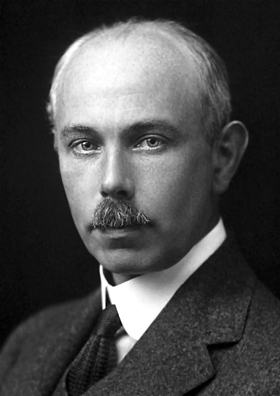
\includegraphics[width=\linewidth]{images/book3/aston.jpg}
\end{minipage}\hspace{0.02\linewidth}%
\begin{minipage}[t]{0.24\linewidth}
\vspace{0pt}
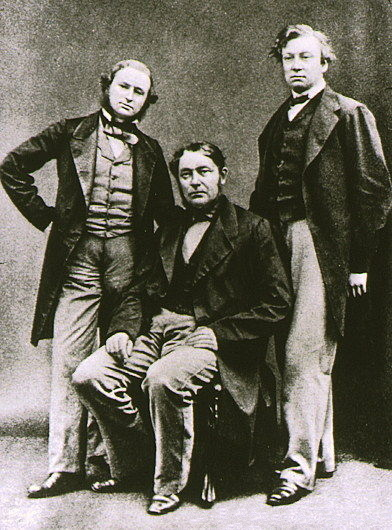
\includegraphics[width=\linewidth]{images/book3/kirchhoff-bunsen.jpg}
\end{minipage}\hfill
\begin{minipage}[t]{0.54\linewidth}
\vspace{0pt}
Gustav Kirchhoff e Robert Bunsen mostraram por volta de 1860 que cada elemento dá suas próprias raias em
uma chama, e descobriram o césio e o rubídio por suas raias desconhecidas. O espectrógrafo de massas de
Francis Aston, a partir de 1919, mostrou que a maioria dos elementos são misturas de isótopos; ele
recebeu o Prêmio Nobel de Química de 1922. (Fotografias: Aston, autor desconhecido, domínio público;
Kirchhoff, Bunsen e Henry Roscoe em 1862, da coleção de Roscoe, domínio público; Wikimedia Commons.)
\end{minipage}
\end{history}

\section{Exercícios}

\begin{exercise}[$\star$]\label{exo:b2:mass-spec-atomic:1}
Dê o $m/z$ de: o \omterm{def:b2:mass-spec-atomic:molecular-ion}{íon molecular} do benzeno \ce{C6H6}; um íon de massa \qty{400}{u} que leva duas
cargas; a molécula protonada da cafeína (\ce{C8H10N4O2}, massa nominal 194) formada por eletrospray.
\end{exercise}

\begin{exercise}[$\star$]\label{exo:b2:mass-spec-atomic:2}
Um composto de C, H, N e O tem um \omterm{def:b2:mass-spec-atomic:molecular-ion}{íon molecular} em $m/z$ 73. O que se pode dizer de seus átomos de
nitrogênio? Proponha uma fórmula.
\end{exercise}

\begin{exercise}[$\star$]\label{exo:b2:mass-spec-atomic:3}
Um agrupamento de \omterm{def:b2:mass-spec-atomic:molecular-ion}{íon molecular} mostra dois picos separados de duas unidades, de alturas quase iguais.
Outro mostra dois picos separados de duas unidades na razão 3 : 1. Que halogênios?
\end{exercise}

\begin{exercise}[$\star$]\label{exo:b2:mass-spec-atomic:4}
Um sal colore uma chama de amarelo; outro de carmim. Identifique os elementos e dê os comprimentos de
onda de suas raias.
\end{exercise}

\begin{exercise}[$\star\star$]\label{exo:b2:mass-spec-atomic:5}
Um hidrocarboneto tem $M$ a 100 \% e $M+1$ a 6.7 \%. Quantos átomos de carbono ele contém?
\end{exercise}

\begin{exercise}[$\star\star$]\label{exo:b2:mass-spec-atomic:6}
Calcule as massas exatas de \ce{CO}, \ce{N2} e \ce{C2H4} e o poder de resolução necessário para separar
cada par.
\end{exercise}

\begin{exercise}[$\star\star$]\label{exo:b2:mass-spec-atomic:7}
O espectro EI da pentan-3-ona mostra picos em 86, 57 (\omterm{def:b2:mass-spec-atomic:spectrum}{pico base}) e 29. Atribua-os.
\end{exercise}

\begin{exercise}[$\star\star$]\label{exo:b2:mass-spec-atomic:8}
O espectro da pentan-2-ona mostra picos em 86, 71, 58 e 43 (\omterm{def:b2:mass-spec-atomic:spectrum}{pico base}). Atribua-os, e explique por
que a pentan-3-ona mostra apenas um pequeno pico em 58.
\end{exercise}

\begin{exercise}[$\star\star$]\label{exo:b2:mass-spec-atomic:9}
Padrões de cobre a 1.0, 2.0, 3.0 e \qty{4.0}{mg/L} dão absorbâncias 0.052, 0.104, 0.155 e 0.207;
uma amostra dá 0.128 (dados do exercício). Calcule sua concentração de cobre.
\end{exercise}

\begin{exercise}[$\star\star\star$]\label{exo:b2:mass-spec-atomic:10}
Em um analisador de tempo de voo, $L = \qty{1.00}{m}$ e $U = \qty{20.0}{kV}$. Calcule o tempo de voo
de um íon monocarregado de massa \qty{1000}{u}, e o tempo que o separa de um íon de \qty{1001}{u}.
\end{exercise}

\begin{exercise}[$\star\star\star$]\label{exo:b2:mass-spec-atomic:11}
Calcule o agrupamento do \omterm{def:b2:mass-spec-atomic:molecular-ion}{íon molecular} do diclorometano, \ce{CH2Cl2}: valores de $m/z$ e intensidades
relativas.
\end{exercise}

\begin{exercise}[$\star\star\star$]\label{exo:b2:mass-spec-atomic:12}
Em ICP-MS, \ce{^{40}Ar^{16}O+} interfere com \ce{^{56}Fe+}. Calcule o poder de resolução necessário
para separá-los, e proponha outra saída.
\end{exercise}

\section{Problema: Um haleto desconhecido}

\begin{problem}[{Problema de fim de semana --- um agrupamento de íon molecular com cloro e bromo, o
número de carbonos, os fragmentos, e uma estrutura verificada contra cada pico}]
\label{pb:b2:mass-spec-atomic:1}
Um líquido incolor, eluído como um único pico em \omterm{def:b2:chromatography:techniques}{cromatografia gasosa}, dá o \omterm{def:b2:mass-spec-atomic:spectrum}{espectro de massas} EI abaixo
(dados do NIST WebBook). Picos principais ($m/z$: intensidade relativa): 156: 14.5; 157: 0.5; 158: 18.6; 159: 0.6; 160:
4.4; 107: 6.7; 109: 6.3; 93: 3.3; 95: 2.9; 77: 59; 79: 18.7; 76: 39.5; 49: 12.9; 51: 4.3; 41: 100; 39:
26.2; 27: 24.6. Abundâncias isotópicas: \ce{^{35}Cl} 0.758, \ce{^{37}Cl} 0.242, \ce{^{79}Br} 0.5069,
\ce{^{81}Br} 0.4931, \ce{^{12}C} 0.989, \ce{^{13}C} 0.011.
% ledger: ms:bromochloropropane, iso:Cl35, iso:Cl37, iso:Br79, iso:Br81, iso:C12, iso:C13, mass:C12, mass:H1, mass:Br79, mass:Cl35

\begin{center}
\begin{tikzpicture}
\begin{axis}[width=0.8\linewidth, height=4.6cm, xmin=20, xmax=170, ymin=0, ymax=112,
  xlabel={$m/z$}, ylabel={intensidade relativa}, label style={font=\small},
  tick label style={font=\scriptsize}, ycomb, xtick={27,41,49,77,93,107,122,156}]
\addplot[omDef, thick] table[x=mz, y=I] {figdata/out/bachelor-2-mass-spectra-d.dat};
\end{axis}
\end{tikzpicture}
\end{center}
% figdata: bachelor-2/mass-spectra.py part d

\medskip
\noindent\textbf{Parte I --- O \omterm{def:b2:mass-spec-atomic:molecular-ion}{íon molecular}.}
\begin{enumerate}
  \item Que picos formam o agrupamento do \omterm{def:b2:mass-spec-atomic:molecular-ion}{íon molecular}? Por que não é um único pico?
  \item Que halogênios sugere um agrupamento de três picos espaçados de 2?
  \item Qual é a massa nominal da forma isotópica mais leve?
  \item O que diz a \omterm{def:b2:mass-spec-atomic:nitrogen-rule}{regra do nitrogênio}?
  \item Subtraia um \ce{^{79}Br} e um \ce{^{35}Cl}: o que resta, e que fragmento hidrocarbonado
        tem essa massa?
  \item Proponha uma fórmula molecular e dê seu grau de insaturação.
\end{enumerate}

\medskip
\noindent\textbf{Parte II --- Carbonos e massa exata.}
\begin{enumerate}[resume]
  \item A partir da razão 157/156, estime o número de carbonos.
  \item Por que essa estimativa é grosseira aqui?
  \item Que formas isotópicas contribuem para o pico em 158?
  \item Calcule a \omterm{def:b2:mass-spec-atomic:exact-mass}{massa monoisotópica} do \omterm{def:b2:mass-spec-atomic:molecular-ion}{íon molecular}.
  \item \ce{C10H20O} também tem massa nominal 156 (exata 156.151). Que poder de resolução separa os
        dois?
  \item O \omterm{def:b2:mass-spec-atomic:molecular-ion}{íon molecular} de um composto com uma ligação C=C e os mesmos halogênios teria uma massa
        nominal diferente?
\end{enumerate}

\medskip
\noindent\textbf{Parte III --- Os fragmentos.}
\begin{enumerate}[resume]
  \item O par 77/79 está na razão 3 : 1. Que átomo foi perdido, e qual é o íon?
  \item Explique o pico em 76.
  \item Atribua o \omterm{def:b2:mass-spec-atomic:spectrum}{pico base} em 41.
  \item Atribua o par 49/51.
  \item Atribua os pares 93/95 e 107/109.
  \item Por que um átomo de bromo é perdido mais facilmente que um átomo de cloro?
  \item O 1-bromo-1-cloropropano daria \ce{CHBrCl+} em 127, 129 e 131. O espectro
        o confirma?
\end{enumerate}

\medskip
\noindent\textbf{Parte IV --- A estrutura.}
\begin{enumerate}[resume]
  \item Proponha a estrutura.
  \item Verifique que ela explica cada pico listado.
  \item Pode ocorrer um \omterm{def:b2:mass-spec-atomic:fragmentation}{rearranjo de McLafferty}? Por quê?
  \item Desenhe o isômero que daria um pico forte em $m/z$ 63/65 e nenhum em 49/51.
  \item Que formas isotópicas formam o pico em 160?
  \item A partir das abundâncias isotópicas, calcule a razão dos picos $M$, $M+2$ e $M+4$ para um
        cloro e um bromo, e compare-a com o espectro.
\end{enumerate}
\end{problem}
